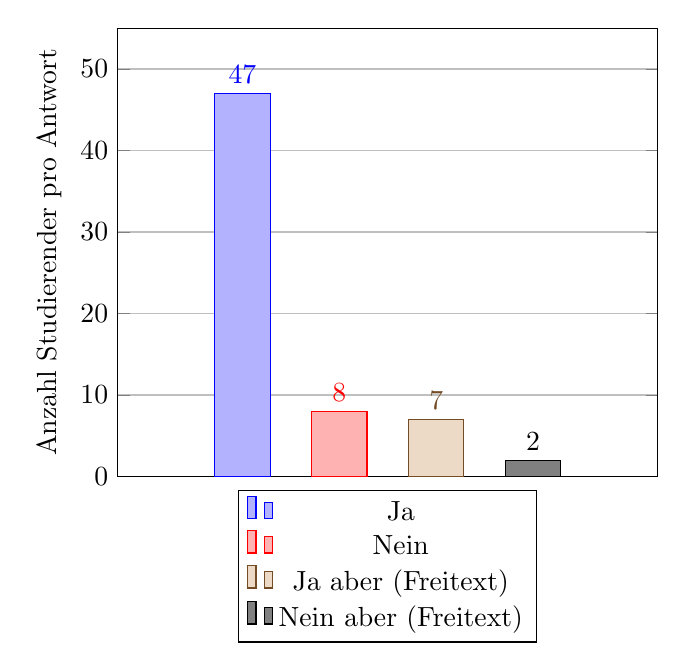
\begin{tikzpicture}
    \begin{axis}[
        x tick label style={
    		/pgf/number format/1000 sep=},
    	ylabel=Anzahl Studierender pro Antwort,
    	enlarge x limits=2,
        ymax=55,
        ymin=0,
    	legend style={at={(0.5,-0.03)},
        anchor=north,legend columns=1},
        ybar,
        bar width=20pt,
        xticklabels={},
        xtick=\empty,
        nodes near coords,
        grid=major,
    ]
    \addplot coordinates {(1,47)};
    \addplot coordinates {(2,8)};
    \addplot coordinates {(3,7)};
    \addplot coordinates {(4,2)};
    
    \legend{Ja, Nein, Ja aber (Freitext), Nein aber (Freitext)}
    \end{axis}
\end{tikzpicture}